\documentclass[a4paper, 11pt]{article}
\usepackage[czech,slovak,english]{babel}
\usepackage[utf8]{inputenc}
\usepackage{url}
\usepackage{fullpage}
\usepackage{hyperref}
\def\UrlBreaks{\do\/\do-}
\usepackage{float}
\usepackage{graphicx}
\graphicspath{ {images/} }

\title{Model domovov dôchodcov}

\begin{document}
\begin{center}
\Large \textbf{Model domovov dôchodcov}
\end{center}
\noindent
\large{\textbf{Modelovanie domova dôchodcov (5)}} \hfill \textbf{Ondrej Kurák}, xkurak00 \\
\today \hfill \textbf{Martin Bažík}, xbazik00 \\


\section{Úvod}
V tejto práci je riešená implentácia modelu\cite[str. 7]{IMS} napĺňania kapacít domovov dôchocov a vývoja demografie obyvateľstva. Na základe vytvoreného modelu a simulačných experimentov\cite[str. 8]{IMS} sa pokúsime vytvoriť predpoklad pre rok naplnenia aktuálnej kapacity domovov dôchodcov v juhomaravskom kraji. Jednotlivé experimenty sa zameriavajú na odhady vývoja aktuálneho stavu zaplnenia domovov dôchodcov.
\subsection{Autori}
\begin{itemize}
\item Martin Bažík (xbazik00)
\item Ondrej Kurák (xkurak00)
\end{itemize}
\subsection{Odborný konzultant}
\begin{itemize}
\item MUDr. Milan Kurák
\end{itemize}
\subsection{Zdroje faktov}
Ako hlavné zdoje faktov boli použité správy z Ústavu zdravotných informácii a štatistýk Českej republiky\cite{demografia}\cite{domovy}, správy Českého štatistického úradu\cite{zomreli} a konzultácia s odborným konzultantom. Všetky zdroje sú uvedené v sekcii \textbf{Zdroje}.  
\subsection{Validita modelu}
Validitu modelu\cite[str. 37]{IMS} pre vývoj demografie obyvatelstva je čiastočne overená na základe porovnávania úmrnosti našeho modulu a výsledkami Českého štatistického úradu\cite{lifet}. Kvôli dĺžke experimentu, presnosť výsledkov s časom klesá.

\section{Rozbor témy a použitých metód/technológií}
Práca sa zaoberá modelom napĺňania kapacít domovov pre dôchodcov a vývojom demografie v juhomoravskom kraji. 

Domov pre dôchodcov je zariadenie, do ktorého prichádzajú klienti po dosiahnutí určitého veku. Pre tento projekt sme zvolili vek 60 rokov, ktorý je možné odvodiť na základe tabuľky \texttt{Důchodový věk}\cite{duchod}. Priemerný vek mužov, ktorý nastúpia do dôchodku od roku 2017 do roku 2044, je 65 rokov. Dôchodkový vek žien však závisí na množstve detí, je však nižší ako vek mužov. Svetová zdravotnícka organizácia WHO klasifikuje ľudí vo veku 60-74 ako skorú starobu\cite{pac}, čo potvrdzuje túto hodnotu.

Hlavným faktorom napĺňania domova dôchodcov je starnutie populácie. Stredná dĺžka života na základe tabuľky \texttt{Vývoj ukazatelů úmrtnosti} \cite[str. 8]{zomreli} rastie, pričom v poslednom meranom roku 2016 dosiahol medziročný nárast o 0,5\%.

Napĺňanie domovov pre dôchodcov taktiež závisí na fakte, koľko percent obyvateľstva chce vstúpiť do domova pre dôchodcov. Tieto hodnoty vychádzajú z počtu príslušníkov jednotlivých vekových kategórií na, ktorý sa v roku 2013 nachádzali v domove dôchodcov\cite{domovy}. Ďalšie hodnoty boli získané po konzultácii s expertom.

Na napĺňanie domovov pre dôchodcov má vplyv aj ich samotná kapacita. Pre tento projekt sme zvolili konštatnú kapacitu, ktorá je pre juhomoravský kraj definovaná na základe tabuľky\cite{miesta}. Súčasný stav tvorí 4128 miest.  

Pre modelovanie demografie populácie sú potrebné dáta o súčasnom stave populácie\cite{demografia} a obsadení domovov pre dôchodcov\cite{domovy}, úmrtnosť jednotlivých vekových kategórii\cite{zomreli}, ako aj pôrodnosť. Nakoľko model obmedzujeme do roku 2040, je pôrodnosť zanedbateľná. Novonarodení jedinci totiž nemôžu dosiahnuť dôchodkový vek vo vymedzenom časovom období. Minimálny vek, pre ovplynvnenie modelu, je 35 rokov.

Jednotlivé dáta sú agregované v päťročných kategóriách a pre tento projekt ich bolo potrebné spracovať pre jednotlivé roky.

\subsection{Použité postupy}
Pre simulačný model\cite[str. 44]{IMS} je využitá diskrétna simulácia\cite[str. 34]{IMS}. Tento model je implementovaný v programovacom jazyku Python. Dôvodom pre využitie programovacieho jazyka Python je možnosť využitia vedeckých knižníc Numpy a Scipy a vizualizačnej knižnice Matplotlib. Pomocou týchto knižníc dokážeme jednoducho aproximovať krivky na výpočet komponentov potrebných pre náš model. Následne vizualizačné knižnice uľahčujú overenie dát pomocou ich vizualizácie v podobe grafov.

\subsection{Použité technológie}
\begin{itemize}
\item Python 3.x \url{https://www.python.org/}
\item Numpy \url{http://www.numpy.org/}
\item SciPy \url{https://www.scipy.org/}
\item Matplotlib \url{https://matplotlib.org/}
\end{itemize}
\subsubsection{Spustenie na serveri Merlin}
Pre spustenie programu na serveri merlin, je potrebné pripraviť virtuálne prostredie s knižnicami Numpy a Scipy. Postup prípravy a spustenia je:
\begin{itemize}
\item Pripravenie virtuálneho prostredia:\\
\texttt{\$ python3 -m venv test-env}
\item Nainštalovanie knižníc Numpy a Scipy:\\
\texttt{\$ test-env/bin/pip3 install scipy}
\item Spustenie programu v virtuálnom prostredí:\\
\texttt{\$ test-env/bin/python3 main.py}
\end{itemize}
Pri tejto konfigurácii sa spustí základná verzia programu, vypisujúca výsledky na štandardný výstup. Pre verziu s vizualizáciou je potrebné spustiť súbor \texttt{ims.ipynb} v programe \texttt{jupyter}.

\section{Koncepcia modelu}
Hlavnou zložkou modelu je predpoveď demografie obyvatelstva. Aby sa dosiahla čo najväčšiu presnosť, je potrebné meniť úmrtnosť obyvatelstva a vhodne rozložiť agregované dáta.

\subsection{Spôsob vyjadrenia modelu}
Model môžeme rozložiť na dve hlavné časti, vekový blok pokrývajúci jednu vekovú kategóriu a vypočítavanie pravdepodobnosti úmrtia.

Vekový blok môžeme vyjadriť ako petriho sieť [Obr 1]. Kde S1 je počet ľudí na začiatku roku, $p(x)$ je pravdepodobnosť úmrtia, S2 je počet ľudí, ktorí prežili daný rok, S3 je počet ľudí, ktorí zomreli v danom roku a C0 je kontrolný stav, pre postupné spúštanie jednotlivých vekových blokov. Takého vekové bloky sú naskladané za sebou pre každú vekovú kategóriu.
\renewcommand{\figurename}{Obr}
\begin{figure}[H]
\centering
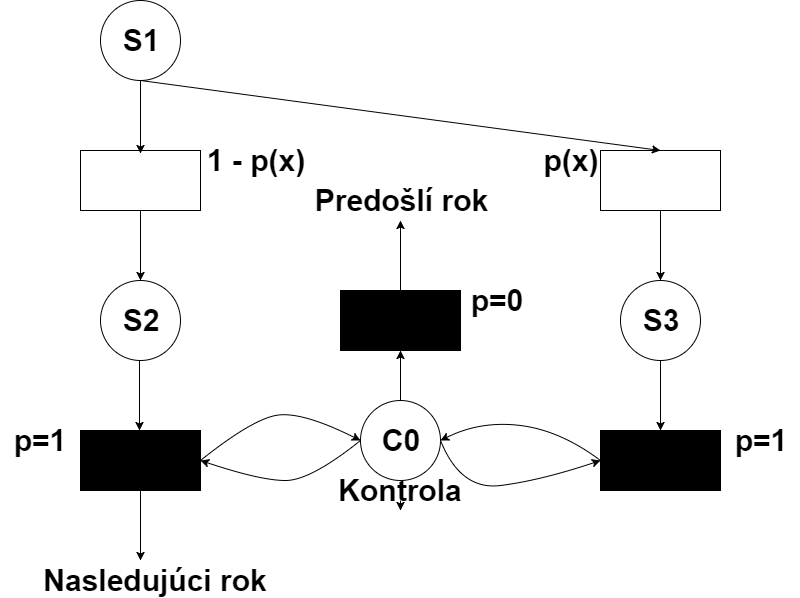
\includegraphics[width=0.5\textwidth]{petri}
\caption{Vekový blok v petriho sieti}
\end{figure}
Počítanie pravdepodobnosti úmrtia sa detailne rozoborá v nasledujúcej časti.


\subsection{Popis konceptuálneho modelu}
Všetky dáta, ktoré je možné pre demografiu obyvatelstva a domovy dôchodcov sú agregované do kategórii po piatich rokoch. Aby bolo možné modelovať jednotlivé zložky je potrbené tieto údaje vhodne rozložiť.

\subsubsection*{Predpovedanie úmrtnosti obyvateľstva a pravdepodobnosti úmrtia}
K úmrtnosti obyvatelsta disponujeme dátami o úmrtnosti pre jednotlivé vekové kategórie (agregovaných po piatich rokoch) od roku 2005. Pravdepobnosť úmrtia následne odvodíme \cite{prob}.

Pre prepovedanie úmrtnosti vekových kategórii aproximujeme na akuálne dáta nelineárnu funkciu pre každú vekovú kategóriu. Funkcia je v tvare:
$$f(x)=\frac{a_0}{x^{a_1} + a_2}$$
Aproximácia prebieha zmenou koeficientov $a_0, a_1, a_2$ metódou najmenších štvorcov\cite{spline}. Daný typ funkcie bol zvolený, pretože dáta majú zostupný charakter a zároveň predpokladáme, že úrtnosť nemôže dosiahnuť 0\%.
\begin{figure}[H]
\centering
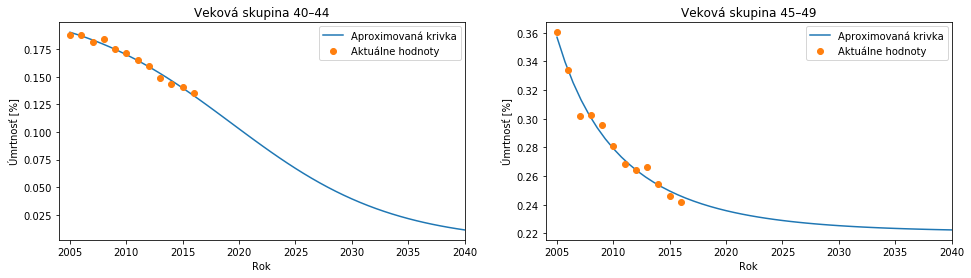
\includegraphics[width=1\textwidth]{exp_1}
\caption{Aproximácia úmrnosti pre vybrané vekové kategórie do roku 2040}
\end{figure}

Aby bolo možné určiť úmrtnosť pre každú vekovú kategóriu (nie kategórie spojené po piatich rokoch, vekové kategórie nad 85 rokov) pomocou predošlých funkcii pre každý sledovaný rok vygenerujeme body pre každú agregovaná vekovú kategóriu. Následne aproximujeme nelineárnu funkciu cez takto vygenerované body. Funkcia je v tvare:
$$f(x) = a_0 * x^a_1 + a_2$$
Aproximácia prebieha zmenou koeficientov $a_0, a_1, a_2$ metódou najmenších štvorcov. Daný typ funkcie bol zvolený, pretože dáta majú vzostupný charakter a konvexný tvar.

Pravdepodobnosť úmrtia pre každú kategóriu vieme následne vypočítať ako 
$$q_x = 1 - \epsilon^{-m_x} $$
kde $q_x$ je pravdepobnosť úmrtia a $m_x$ je percentuálna úmrtnosť \cite{prob}.
\begin{figure}[H]
\centering
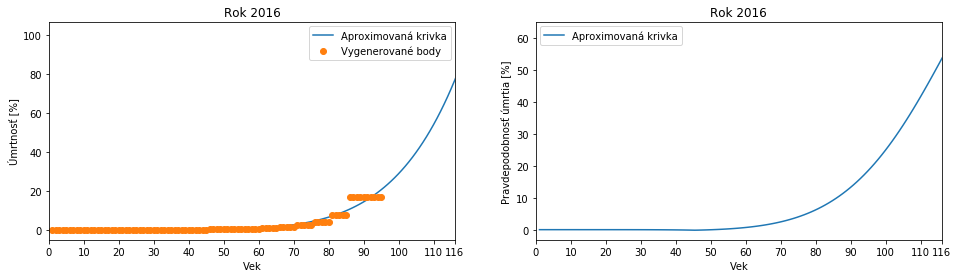
\includegraphics[width=1\textwidth]{exp_2}
\caption{Úmrtnosť a pravdepodobnosť smrti pre rok 2016}
\end{figure}

\subsubsection*{Počiatočné rozloženie obyvateľstva}
Kedže počiatočný stav jednotlivých vekových kategórii obyvatelstva je tak isto agregovaný po piatich rokoch robíme jeho rozloženie na 5 častí. Aby rozloženie čo najviac zodpovedalo realite, vychádzame z niekoľkých prepokladov:
\begin{enumerate}
\item Počet narodených detí sa päťročné obdobie mení minimálne.
\item Počet ľudí v nasledujúcej vekovej kategórii by mal byť menší o počet ľudí, ktorí umreli v poslednom roku.
\end{enumerate}
Tieto predpoklady zväčša platia na vekových skupinách od 35, čo je hlavná zložka nami sledovaného obyvateľstva.

Počet ľudí pre agregovanú vekovú kategóriu vyjadriť ako $y = x_{k} + x_{k+1} + x_{k+2} + x_{k+3} + x_{k+4}$, kde $x_0$ až $x_4$ sú počty ľudí jednotlivých vekových kategórii. Za pomoci predpokladov a percentuálnej úmrtnosti pre jendotlivé vekové kategórie vieme vyjadriť v tvare $x_{k+1}=x_{k}*P(k)$ kde $P(k)$ je doplnok k percentuálnej úmrtnosti danej vekovej kategórie. Následne dokážeme vyjadriť počet ľudí pre agregované kategórie ako:
$$y = x_k*(1 + P(k)*(1 + P(k+1)*(1 + P(k+2) * (1 + P(k+3)))))$$
Týmto spôsobom vieme rozdeliť obyvatelstvo tak, aby sme zachovali počet ľudí pre agregovanú kategóriu a zároveň ich rozdelili s dôrazom na úmrtnosť.
\begin{figure}[H]
\centering
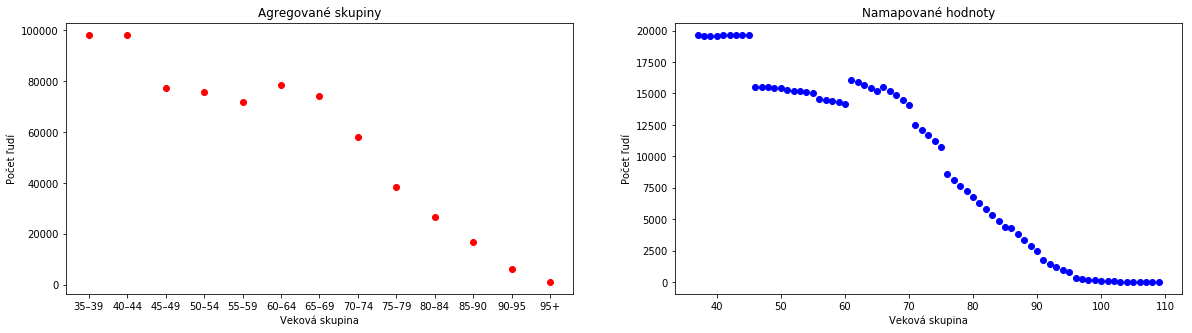
\includegraphics[width=1\textwidth]{exp_3}
\caption{Rozloženie obyvateľstva}
\end{figure}

\section{Architektúra simulačného modelu/simulátoru}
Model je implementovaný v programovacom jazyku Python3 a využíva objektové paradigma. Program sa skladá z viacerích tried, pričom zádkladnou triedou je \texttt{Controller}.

\subsection{Mapovanie abstraktného modelu na simulačný}
Každá trieda implementuje jednu časť abstraktného modelu.

Trieda \texttt{Probs} zastrešuje výpočet pravdepodobnosti úmrtia pre jednotlivé kategórie. Na základe údajov z minulosti, vytvorí predpoklad pre vývoj pravdepodobnosti úmrtia pre každú vekovú kategóriu.

Trieda \texttt{Age} zastrešuje jeden vekový blok modelu. Pri použití jej metódy \texttt{resolve\_year()} podľa pravdepodobnosti úmrtia určí koľko ľudí pokračuje do vyššej vekovej kategórie.

Trieda \texttt{Controller} zastrešuje celý model. Trieda inicializuje bloky pre jednotlivé vekové kategórie a prvotné rozdelenie obyvateľstva. Následne sa stará o prechod medzi rokmi a predávanie informácii o počte obyvateľov medzi jednotlivými blokmi vekovými kategórie. Vekové kategórie sa vyhodnocujú od najstaršej po najmladšiu, aby sa zabezpečilo vyprázdnenie vyššej kategórie pred príchodom nových dát.

\section{Podstata simulačných experimentov a ich priebeh}
Cieľom experimentov je zistiť potrebné kapacity pre domovy dôchodcov do roku 2040. Kedže je problém zistiť presné hodnoty záujemcov o pobyt v domove, pretože každý záujemca si môže podať ľubovoľný počet prihlášok, v experimentoch budeme vychádzať z dát o zaplnení domovov dôchodcov zistených Českým štatisktickým úradom v roku 2013 \cite{domovy2013} a z rozhovoru s odborným konzultantom.
\subsection{Postup experimentov}
Pre každý experiment podľa jeho charakteru sa zvolia zistené hodnoty o percentuálnom zastúpení jednotlivých vekových kategórii v domovoch dôchodcov. Následne sa pre každý rok sleduje stav zaplnenia, aby bolo možné nájsť rok, v ktorom sa prečerpajú aktuálne kapacity.
\subsection{Experimenty}
\subsubsection{Experiment 1}
Experiment 1 sa zameriava na spodný odhad pre potrebné kapacity. Pri rozhovore s odborným konzultatom nám bolo potvrdené, že postupne sa zvyšuje záujem o pobyt v domovoch, tak ako tomu je i zahraničí. Rast u nás však nie je kvôli chýbajucim údajom možné presne namerať. Preto ako spodný odhad je vhodné použiť posledné známe hodnoty. Tým pádom hodnoty pre percentuálne zastúpenie vekových kategórii v domovoch dôchodcov pôužijeme údaje zistené Českým štatistickým úradom z roku 2013 \cite{domovy2013} pre Juhomoravský kraj. Dosiahnuté výsledky môžeme vidieť v grafe nižšie \ref{exp_4}[Obr 5]. Z experimentu nám vyplýva, že aktuálne kapacity domovov dôchodcov budú prečerpané približne v roku 2026. 
\begin{figure}[H]
\centering
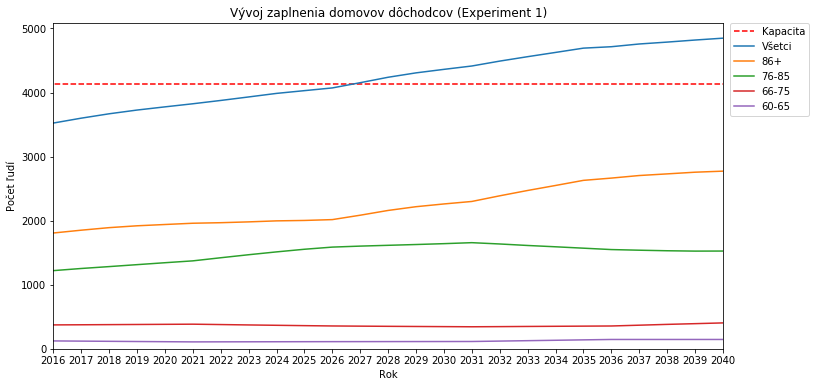
\includegraphics[width=0.8\textwidth]{exp_4}
\caption{Vývoj zaplnenia domovov dôchodcov\label{exp_4}}
\end{figure}

\subsubsection{Experiment 2}
Experiment 2 sa zameriava na kapacity vyvodené z priemeru Českej republiky. Aby sme dokázali ukázať situaciu zvýšenie záujmu zvýšime údaje pre Juhomoravský kraj použité v experimnete 1 na priemer Českej republiky. Pri rozhovore s odborným konzultantom bolo zhodnotené, že takáto zmena by mohla reprezentovať zvyšovanie záujmu o domovy dôchodcov. Výsledky experimentu je možné pozorovať v grafe nižšie [Obr 6]. Pri zvýšení hodnôt, sme sa dostali do prečerpania približne medzi rokmi 2019-2020.
\begin{figure}[H]
\centering
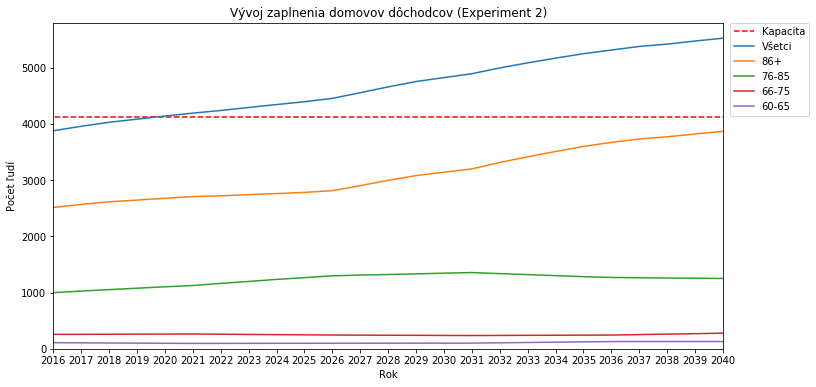
\includegraphics[width=0.8\textwidth]{exp_5}
\caption{Vývoj zaplnenia domovov dôchodcov}
\end{figure}

\subsubsection{Experiment 3}
Experiment 3 sa zameriava na počet ľudí nad 85, ktorí starostlivosť v domove dôchodcov budú reálne potrebovať. Podľa údajov zo zahraničia, bude potrebovať približne 20 percent dôchodcov vo veku nad 85 rokov starostlivosť domova dôchodcov \cite{amerika}. Kedže údaj pre Českú republiku neexistuje, približný údaj sme zistili u odborného konzultanta. Podľa údajov o jeho pacientoch z populácie nad 85 rokov, bude potrebovať starostlivosť v domove dôchodcov niečo medzi 16-17 percent populácie. Výsledok experimentu, pre túto vekovú kategóriu môžeme vidieť v grafe nižšie [Obr 7]. K prečerpaniu kapacít dochádza okolo roku 2019. V tomto experimente, sa ráta ale iba ľudmi nad 85 rokov, ktorí podľa predošlých experimentov tvoria iba 40 percent obyvateľov domovov dôchodcov. Z toho vyplýva, že reálna potreba bude oveľa vačšia.
\begin{figure}[H]
\centering
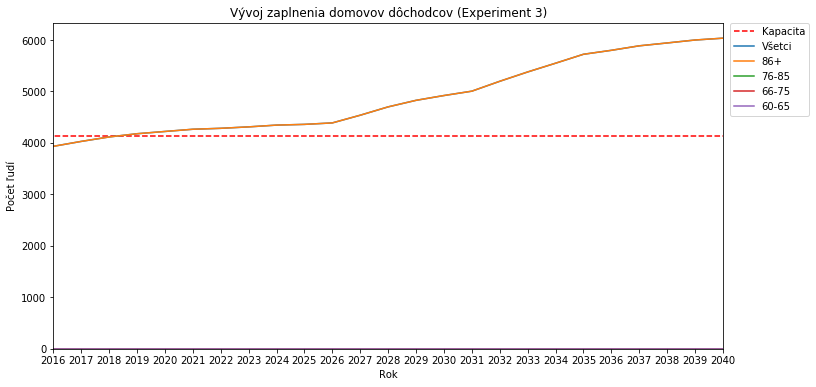
\includegraphics[width=0.8\textwidth]{exp_6}
\caption{Vývoj zaplnenia domovov dôchodcov}
\end{figure}

\subsection{Záver experimentov}
Pomocov experimentov sme stanovili približný odhad na na naplnenie kapacít domovov dôchodcov, v najmiernejšom možnom prípade (Experiment 1). Zároveň sme úkázali nami predpokladaný vývoj naplnenia kapacít (Experiment 2) a ukážku potrebných miest v domovoch dochodcov pre ľudí, ktorí túto starostlivosť budú potrebovať (Experiment~3).

\section{Zhrnutie simulačných experimentov a záver}
Na základe exprimentov dokážeme zhodnotiť, že aktuálne kapacity domovov dôchodcov v Juhomoravskom kraji sú nedostatočné na dlhodobejšie udržanie, aj za predpokladu nezýšenia aktuálneho záujmu.

Za ideálnych podmienk (nezvýšenie zájmu o domovy dôchodcov) dôjde k úplnému napleniu kapacít v roku 2026. Pokiaľ by sa záujem zvýšil na celočeský priemer, k naplneniu by došlo medzi rokmi 2019-2020. 

\newpage
\renewcommand\refname{Zdroje}
\begin{thebibliography}{9}
\bibitem{IMS} Peringer,P.: Modelování a simulace. FIT VUT, [ cit. 29. novembra 2017 ]. Dostupné na: \url{https://www.fit.vutbr.cz/study/courses/IMS/public/prednasky/IMS.pdf}

\bibitem{demografia} Kolektív autorov: Počty obyvatel v okresech ČR dle 5ti letých věkových kategorií. Opendata.cz, [ cit. 27. novembra 2017 ]. Dostupné na: \url{https://linked.opendata.cz/dataset/czso-demography-in-regions-czech-republic-age-categories}

\bibitem{domovy2013} Kolektív autorov: 	Senioři v ČR, [ cit. 27. novembra 2017 ]. Dostupné na: \url{https://www.czso.cz/csu/czso/seniori-v-cr-2014-2gala5x0fg}

\bibitem{domovy} Kolektív autorov: Zařízení sociálních služeb a domy s pečovatelskou službou v okresech ČR. Opendata.cz, [ cit. 27. novembra 2017 ]. Dostupné na: \url{https://linked.opendata.cz/dataset/czso-social-service-facilities}

\bibitem{JM_demografia} Kolektív autorov: Juhomoravský kraj. Wikipédia, [ cit. 27. novembra 2017 ]. Dostupné na: \url{https://sk.wikipedia.org/wiki/Juhomoravsk%C3%BD_kraj}

\bibitem{zomreli} Kolektív autorov: Zemřelí 2016. ÚZIS, 2017, [ cit. 27. novembra 2017 ]. Dostupné na:
\url{http://uzis.cz/publikace/zemreli-2016}

\bibitem{populacia} Kolektív autorov: Obyvatelstvo Česka. Wikipédia, [ cit. 27. novembra 2017 ]. Dostupné na: \url{https://cs.wikipedia.org/wiki/Obyvatelstvo_%C4%8Ceska#Popula.C4.8Dn.C3.AD_statistiky}

\bibitem{miesta} WWW stránka: Domovy pro seniory. GERONTOLOGIE, [ cit. 27. novembra 2017 ]. Dostupné na: 
\url{http://www.gerontologie.cz/showdoc.do?docid=30&typzar=DDP&kraj=Jihomoravsk%FD}

\bibitem{duchod} WWW stránka: Starobní důchody. ČSSZ, [ cit. 29. novembra 2017 ]. Dostupné na: 
\url{http://www.cssz.cz/cz/duchodove-pojisteni/davky/starobni-duchody.htm}

\bibitem{prob} Life Tables for the Czech Republic, Cohesion Regions, and Regions [ 30. novembra 2017 ] Dostupné na: \url{https://www.czso.cz/documents/10180/45948540/13006317ma.pdf/683f399f-f01c-4399-99af-4dd1f04bdac0?version=1.0}

\bibitem{lifet} Life Tables for the Czech Republic, Cohesion Regions, and Regions [ 4. decembra 2017 ] Dostupné na:
\url{https://www.czso.cz/csu/czso/life-tables-for-the-czech-republic-cohesion-regions-and-regions-2015-2016}

\bibitem{pac} PACOVSKÝ, V.: O stárnutí a stáří. 1. vyd. Praha: Avicenum, 1990. ISBN 80-201-0076-8

\bibitem{manualx} Kolektív autorov: Manual X: Indirect Techniques for Demographic Estimation. New York: UNITED NATIONS, 1983. Dostupné na:
\url{http://www.un.org/esa/population/publications/Manual_X/}

\bibitem{spline} Smith L.,Hyndman R. J.,Wood N.: Spline Interpolation for Demographic Variables:
The Monotocity Problem. 
\url{https://link.springer.com/content/pdf/10.1007%2FBF03032212.pdf}

\bibitem{amerika} The Centers for Medicare \& Medicaid Services: Nursing Home Data Compendium 2015 
\url{https://www.cms.gov/Medicare/Provider-Enrollment-and-Certification/CertificationandComplianc/Downloads/nursinghomedatacompendium_508-2015.pdf}
\end{thebibliography}



\end{document}
